\documentclass[11pt,letterpaper,twocolumn]{article}
\usepackage[margin=0.65in,columnsep=0.25in]{geometry}
\usepackage{pgfplots}
\pgfplotsset{compat=1.18}
\usepackage{booktabs}
\usepackage{amsmath}
\usepackage{caption}
\usepackage{microtype}
\setlength{\textfloatsep}{7pt}
\setlength{\floatsep}{5pt}
\usepackage{titlesec}
\usepackage{float}

\setlength{\parindent}{0pt}
\setlength{\parskip}{3pt}
\captionsetup{font=small,labelfont=bf,skip=3pt}
\titlespacing*{\section}{0pt}{7pt}{3pt}
\begin{document}
\twocolumn[{
\begin{center}
{\Large\bfseries Performance Evaluation of Parallel Prefix Sum Algorithms with OpenMP\par}
\vspace{4pt}
{\small CS 431 Homework 2 \par}
\end{center}
\vspace{0pt}
}]
\section*{Algorithms}
A prefix sum computes $P[i]=\sum_{j=0}^{i}A[j]$ for an input array $A$.
The provided serial implementation accumulates values sequentially in $O(n)$ work and $O(n)$ span. Its dependency on previous loop prevents direct parallelization.

\textbf{Parallel 1 (increasing-stride scan):} Each iteration combines partial sums at offsets $1,2,4,\ldots$. Elements within each round are independent when separate read/write buffers are used. The algorithm performs $O(n\log n)$ work in $O(\log n)$ parallel rounds.

\textbf{Parallel 2 (tree-based scan):} An up-sweep builds partial sums in a balanced binary tree, a down-sweep propagates offsets to form the scan. This yields $O(n)$ work with $O(\log n)$ span. 

\section*{Experiment}
Input arrays contained $2^{20}=1{,}048{,}576$ and $2^{23}=8{,}388{,}608$ integers with fixed random seed 5. The skeleton's TSC-based timer measured each routine separately. Table~\ref{tab:times} reports single-run results; Figs.~\ref{fig:small} and~\ref{fig:large} show the same measurements. Timings include each implementation's allocation and OpenMP overhead.

\begin{table}[H]
\centering
\caption{Measured runtimes in ms.}
\label{tab:times}
\setlength{\tabcolsep}{4pt}
\footnotesize
\begin{tabular}{@{}ccrrr@{}}
\toprule
$n$ & Threads & Serial & $O(n\log n)$ & Tree $O(n)$ \\
\midrule
$2^{20}$ & 1 & 2.229 & 7.452 & 2.836 \\
$2^{20}$ & 2 & 2.336 & 7.746 & 2.485 \\
$2^{20}$ & 4 & 2.121 & 6.961 & 2.357 \\
$2^{23}$ & 1 & 8.363 & 73.331 & 31.682 \\
$2^{23}$ & 2 & 9.620 & 66.392 & 24.826 \\
$2^{23}$ & 4 & 8.743 & 60.057 & 22.753 \\
\bottomrule
\end{tabular}
\end{table}

\begin{figure}[H]
\centering
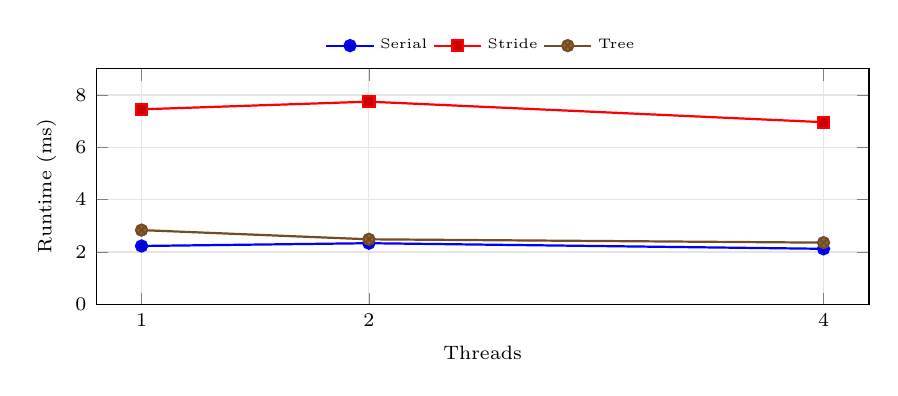
\begin{tikzpicture}
\begin{axis}[
 width=0.94\columnwidth,height=1.80in,
 xlabel={Threads},ylabel={Runtime (ms)},
 xtick={1,2,4},xmin=0.8,xmax=4.2,
 ymin=0,ymax=9,
 grid=major,grid style={gray!20},
 tick label style={font=\scriptsize},label style={font=\scriptsize},
 legend style={font=\tiny,at={(0.5,1.02)},anchor=south,legend columns=3,draw=none},
 every axis plot/.append style={thick,mark=*}]
\addplot coordinates {(1,2.22945) (2,2.33558) (4,2.12115)};
\addplot coordinates {(1,7.45187) (2,7.746) (4,6.96077)};
\addplot coordinates {(1,2.83639) (2,2.48451) (4,2.35735)};
\legend{Serial,Stride,Tree}
\end{axis}
\end{tikzpicture}
\vspace{-7pt}
\caption{Runtime versus threads at $n=2^{20}$.}
\label{fig:small}
\end{figure}

\begin{figure}[H]
\centering
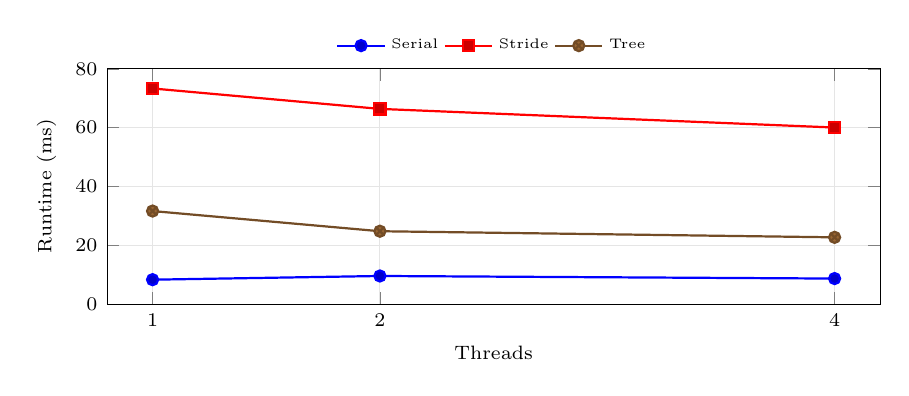
\begin{tikzpicture}
\begin{axis}[
 width=0.94\columnwidth,height=1.80in,
 xlabel={Threads},ylabel={Runtime (ms)},
 xtick={1,2,4},xmin=0.8,xmax=4.2,
 ymin=0,ymax=80,
 grid=major,grid style={gray!20},
 tick label style={font=\scriptsize},label style={font=\scriptsize},
 legend style={font=\tiny,at={(0.5,1.02)},anchor=south,legend columns=3,draw=none},
 every axis plot/.append style={thick,mark=*}]
\addplot coordinates {(1,8.36329) (2,9.61973) (4,8.74308)};
\addplot coordinates {(1,73.3314) (2,66.3915) (4,60.0568)};
\addplot coordinates {(1,31.6824) (2,24.8258) (4,22.7534)};
\legend{Serial,Stride,Tree}
\end{axis}
\end{tikzpicture}
\vspace{-7pt}
\caption{Runtime versus threads at $n=2^{23}$.}
\label{fig:large}
\end{figure}

\section*{Results and Discussion}
Increasing threads from 1 to 4 reduced the $O(n\log n)$ runtime from 73.331 to 60.057 ms (\textbf{1.22$\times$} speedup) and the tree-based runtime from 31.682 to 22.753 ms (\textbf{1.39$\times$}). The tree-based algorithm was \textbf{2.64$\times$ faster} than the increasing-stride algorithm at four threads on $2^{23}$ elements.

The serial baseline in these measurements performed the best. At $2^{23}$ elements and four threads, the serial routine took 8.743 ms versus 22.753 ms for the tree scan and 60.057 ms for the increasing-stride scan. Synchronization across tree levels, memory traffic, repeated OpenMP work-sharing regions, and temporary storage can offset the benefit of a shorter span.

For $n=2^{23}$ and four threads, the
increasing-stride algorithm achieved
\[
S_{\mathrm{stride}}(4)
=\frac{73.331}{60.057}
\approx 1.22.
\]

The tree-based algorithm achieved
\[
S_{\mathrm{tree}}(4)
=\frac{31.682}{22.753}
\approx 1.39.
\]

\section*{Conclusion}
Both implementations passed correctness checks. The work-efficient tree scan consistently beat the increasing-stride version, and both improved with more threads on the larger input. However, the serial scan remained fastest, illustrating the practical importance of synchronization and memory overhead.
\end{document}